\documentclass[12pt]{article}
\usepackage[T1]{fontenc}
%\usepackage[latin9]{inputenc}
\usepackage[utf8]{inputenc}
\usepackage[english]{babel}
\usepackage{amsmath}
%\usepackage{halloweenmath}
\usepackage{amsfonts}
\usepackage{amssymb}
%\usepackage{setspace}
\usepackage{rotating}
\usepackage{graphics}
\usepackage{eurosym}
\usepackage[round]{natbib}
%\usepackage{graphicx}
%\usepackage{float} 				%allows you to float images
\usepackage{latexsym}
%\usepackage{bbding}
%\usepackage {moresize}
\usepackage{listings}
\usepackage{bbding}
\usepackage{blindtext}
\usepackage{hhline}
\usepackage{tikz}
\usetikzlibrary{trees}
%\usetikzlibrary{shapes,backgrounds}
%\usepackage{pgfplots}
%\usetikzlibrary{arrows}
\usepackage{enumitem}
%\doublespacing
%\usepackage{geometry}
\usepackage{amsthm}
\usepackage{color}
%\usepackage{array,multirow}
\usepackage{subcaption}
%\usepackage{pst-plot}
%	\psset{xunit=15mm}
%\geometry{verbose,tmargin=1in,bmargin=1in,lmargin=.5in,rmargin=.5in}
\setlength{\parskip}{\bigskipamount}
\setlength{\parindent}{0pt}
\usepackage{multicol}


\newenvironment{problem}[3][Problem]{\begin{trivlist}
\item[\hskip \labelsep {\bfseries #1}\hskip \labelsep {\bfseries #2.}]}{\end{trivlist}}

\newcommand{\barr}{\bar{r}}
\newcommand{\ddx}{\frac{d}{dx}}
\newcommand{\infsum}{\sum_{n=1}^{\infty }}

\title{Problem Set 11 \thanks{Problems:13.1, 13.5, 13.6, 13.11, 13.25}}
\author{Ian McGroarty \\
	Course Number: 555.444 \\
}
\date{November 12, 2019}

\begin{document}

\maketitle
%%%%%%%%%%%%%%%%%%%%%%%%%%%%%%%%%%%%%%%%%%%%%%%%%%%%%%%%
%%%%%%%%%%%%%%%%%%%%%%%%%%%%%%%%%%%%%%%%%%%%%%%%%%%%%%%%
%%%%%%%%%%%%%%%%%%%%%%%%%%%%%%%%%%%%%%%%%%%%%%%%%%%%%%%%

\newpage
\begin{problem}{15.4}. Calculate the price of a three-month European put option on a non-dividend-paying stock
with a strike price of \$50 when the current stock price is \$50, the risk-free interest rate is
10\% per annum, and the volatility is 30\% per annum. This means that $S_0=50, K=50, r=0.1, \sigma = 0.3, T=0.25$
\begin{align*}
d_1 &= \frac{ln(S_0/K) + (r-\sigma^2/2)(T)}{\sigma \sqrt{T-t}}  && \text{(pg 334)} \\
 &= \frac{ln(50/50) + (0.1-(0.3)^2/2)(0.25)}{0.3 \sqrt{0.25}}  \\
d_1 &= 0.24167 \\
d_2 &= d_1 - \sigma \sqrt{T} && \text{Luenberger (pg. 334)}\\
&= 0.24167 - 0.3 \sqrt{0.25} \\
d_2 &= 0.091667 \\
Ke^{-rT} &= 50\cdot e^{-0.025} = 48.765 && \text{Eqn. 15.19 (pg. 333)} \\
p &= Ke^{-rt}\cdot N(-d_2) - S_0\cdot N(-d_1) && \text{Eqn 15.21 (pg. 333)} \\
&= 48.765 \cdot N(-0.091667) - 50 \cdot N(-0.24167) \\
&= 48.765 \cdot (0.4634) - 50 \cdot (0.4045) \\
p &= 2.3
\end{align*}
\end{problem}

\begin{problem}{15.5}. What difference does it make to you calculations in Problem 15.4 if a dividend of \$1.50 is expected in two months. 

Well the present value of the dividend is $1.50\cdot e^{-0.025} =1.496$. We now need to take this out of our $S_0$, I don\rq{}t fully understand why?? so $S_0 - 50-1.496 = 48.504$. We see below that the price of the put option increases with the dividend. 
\begin{align*}
d_1 &= \frac{ln(48.504/50) + (0.1-(0.3)^2/2)(0.25)}{0.3 \sqrt{0.25}}  = 0.03915 \\
d_2 &= 0.03915  - 0.3 \sqrt{0.25} = -0.111 \\
p &= 48.765 \cdot N(0.111) - 48.504 \cdot N(-0.03915) \\
p &= 3.04
\end{align*} 
\end{problem}

\newpage
\begin{problem}{15.11}. I\rq{}m not entirely sure how to use the risk neutral valuation in it\rq{}s purest form here. But here we go. Following Section 15.7 (pg 332-333): First, assume that the expected return from the underlying asset is the risk free rate. 
\begin{align*}
\mu &= r \\
\text{ Second  } & \text{calculate the expected payoff: } \\
ln S_T &~\sim \Phi [ ln S_0 + (\mu - \frac{\sigma^2}{2})T, \sigma^2T] && \text{Eqn 14.19/15.3 (pg 313/320)} \\ 
&\implies  E(ln S_T) = ln S_0 + (\mu - \frac{\sigma^2}{2})T \\
&= \implies \hat{E}(ln S_T) = ln S_0 + (r - \frac{\sigma^2}{2})T && \text{Risk Neutral} \\
f &= e^{-rT}\hat{E} && \text{Discounted to today} \\
f&= e^{-rT}( ln S_0 + (r - \frac{\sigma^2}{2})T) \\ 
\text{Confirm  }& \text{that this satisfies 15.16} \\
rf &= \frac{\partial f}{\partial t} + rS\frac{\partial f}{\partial S} + \frac{1}{2} \sigma^2 S^2\frac{\partial^2 f}{\partial S^2} && \text{Eqn. 15.16 (pg 330)} \\
\frac{\partial f}{\partial t} &= -r( e^{-rT}( ln S_0 + (r - \frac{\sigma^2}{2})T)) - (e^{-rT}(r-\frac{\sigma^2}{2}) \\
\frac{\partial f}{\partial S} &= \frac{e^{-rT}}{S} \\
\frac{\partial^2 f}{\partial S^2} &= -\frac{e^{-rT}}{S^2} \\
rf &= -r( e^{-rT}( ln S_0 + (r - \frac{\sigma^2}{2})T)) \\
   &- (e^{-rT}(r-\frac{\sigma^2}{2}) + rS\frac{e^{-rT}}{S} - \frac{1}{2} \sigma^2 S^2 \frac{e^{-rT}}{S^2}\\
rf &= -r e^{-rT}( ln S_0 + (r - \frac{\sigma^2}{2})T) \\
   &- e^{-rT}[(r-\frac{\sigma^2}{2}) + (r - \frac{ \sigma^2}{2})]\\
rf &= -r e^{-rT}( ln S_0 + (r - \frac{\sigma^2}{2})T) && \text{We are satisfied}\\
\end{align*}
\end{problem}

\begin{problem}{15.13}. Calculate the price of a three-month European put option on a non-dividend-paying stock
with a strike price of \$50 when the current stock price is \$52, the risk-free interest rate is
12\% per annum, and the volatility is 30\% per annum. This means that $S_0=52, K=50, r=0.12, \sigma = 0.3, T=0.25$ Since this is essentially the same format of 15.4. 
\begin{align*}
d_1 &= \frac{ln(S_0/K) + (r+\sigma^2/2)(T)}{\sigma \sqrt{T-t}}  && \text{(pg 334)} \\
 &= \frac{ln(52/50) + (0.12-(0.3)^2/2)(0.25)}{0.3 \sqrt{0.25}}  \\
d_1 &= 1.934 \\
d_2 &= d_1 - \sigma \sqrt{T} && \text{Luenberger (pg. 334)}\\
&= 1.934 - 0.3 \sqrt{0.25} \\
d_2 &= 1.874 \\
c &= S_0\cdot N(d_1) - K\cdot e^{-rt} \cdot N(d_2) && \text{Eqn 15.20 (pg. 333)} \\
&= 52 \cdot N(1.934_ - 50 \cdot e^{-0.12*0.25} \cdot N(1.874) \\
c &= 3.575
\end{align*}
\end{problem}

\begin{problem}{15.15}. Consider an American call option on a stock. $S_0 = 70, r= 0.10, K=65, \sigma = 0.32, T=0.666$ Dividend after 3 and 6 months. 
It is never optimal to exercise before 3 months if:
\begin{align*}
D_i &\leq K[1-e^{-r(t_{i+1}-t_i)}] && \text{Eqn. 15.25 (pg 343)} \\
D_1 &\leq 65\cdot [1-e^{-0.1((6/12)-(3/12))}] \\
\$ 1  &\leq 1.604 &&\text{15.25 holds} \\
D_2 &\leq 65\cdot [1-e^{-0.1((8/12)-(6/12))}] \\
\$ 1 &\leq 1.074 &&\text{15.25 holds}
\end{align*}
Since 15.25 holds for both times corresponding to all dividends, it is never optimal to exercise the call and thus it can be treated as a European call option. 
\end{problem}

\newpage
\begin{problem}{15.17}. $N`(x) = \frac{1}{\sqrt{2\pi }}e^{-x^2/2}$ is the probability density function for a standard normal distribution (pg 19.2). For part (b),(d),(f) see the photos. I knew if I typed it I\rq{}d miss something so I had to write it out. 
\begin{align*}
\text{(c):  } d_1 &= \frac{ln(S_0/K) + (r+\sigma^2/2)(T)}{\sigma \sqrt{T-t}}  && \text{(pg 334)} \\
\text{Let } a&= \frac{(r+\sigma^2/2)(T)}{\sigma \sqrt{T-t}} \\ 
\frac{\partial d_1}{\partial S} &=  \frac{d}{dS}ln(S/K) \cdot \frac{1}{\sigma \sqrt{T-t}} + a \\
&= \frac{1}{S \cdot  \sigma \sqrt{T-t}} \\
&= \frac{\partial d_2}{\partial S} &&\text{pretty clearly they will be the same} \\
\text{(e):  }c &= SN(d_1) - Ke^{-r(T-t)N(d_2)} \\
\frac{\partial c}{\partial S} &= N(d_1) &&\text{Trivial Solution} \\
\end{align*}
(g):  As $t\rightarrow T \implies \sqrt{T-t} \rightarrow 0 \implies (d_1,d_2) \rightarrow \pm \infty \implies N(d) \rightarrow (0,1).$ If 0 then c=0. If 1 then c= S-K. 


\includegraphics[width=\linewidth]{mod11_p1517b.png}
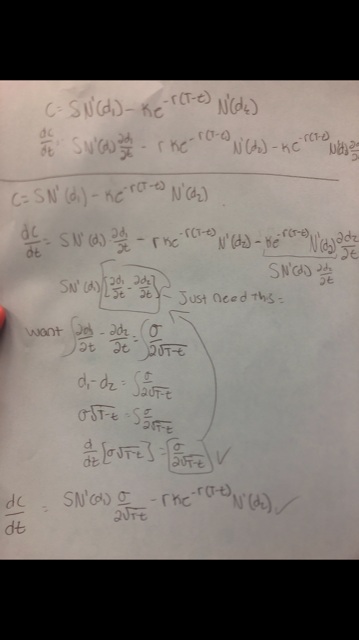
\includegraphics[width=\linewidth]{mod11_p1517d.png}
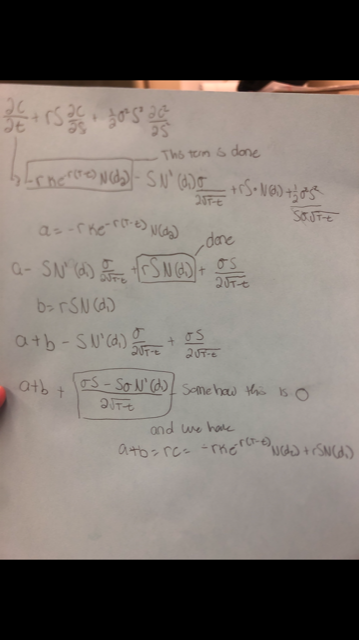
\includegraphics[width=\linewidth]{mod11_p1517f.png}
\end{problem}

\begin{problem}{15.28}.  See Photo. \\
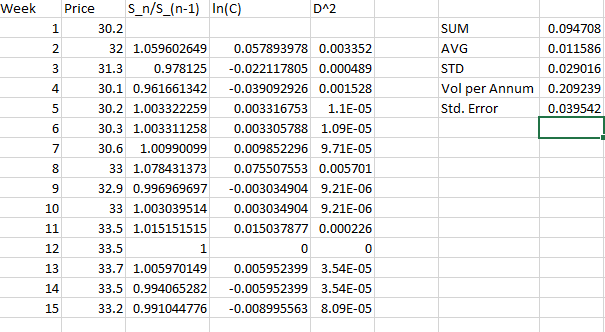
\includegraphics[width=\linewidth]{mod11_p1528.png}
\end{problem}
\end{document}